\documentclass{beamer}

%\usepackage[utf8x]{inputenc}


\usepackage{default}
%\usepackage[english]{babel}

\usepackage{amsmath}
\usepackage{amsthm, amsfonts, amssymb}%fortmattazione teoremi, ecc
\usepackage{bbm}%simboli degli insiemi
\usepackage{mathrsfs}%fornisce un \mathscr, alternativo a \mathcal

\usepackage{fancybox}

\usepackage{biblatex}


\usepackage{listings} %Per inserire codice
%\usepackage[usenames]{color} 
\usepackage{color}

%\definecolor{mygreen}{rgb}{0,0.6,0}

\usepackage{graphicx}

\usepackage{tikz}
\usetikzlibrary{trees,matrix}

%%%
%Definizione nuovi comandi
%%%
\newcommand{\Q}{\mathbb{Q}}
\newcommand{\R}{\mathbb{R}}
\newcommand{\N}{\mathbb{N}}
\newcommand{\Z}{\mathbb{Z}}
\newcommand{\C}{\mathbb{C}}

% %NARE, CARE, ecc.
% \newcommand{\nare}{\mathrm{NARE}}
% \newcommand{\care}{\mathrm{CARE}}
% \newcommand{\gcare}{\mathrm{GCARE}}
% \newcommand{\mnare}{\mathsf{M}-\mathrm{NARE}}
% \newcommand{\adi}{\mathrm{ADI}}
% \newcommand{\cfadi}{\mathrm{C}\mathrm{f}-\mathrm{ADI}}
% \newcommand{\fadi}{\mathrm{f}-\mathrm{ADI}}

%trasposta:
\newcommand{\tras}[1]{#1^{\mathrm{T}}}
%trasposta e coniugata
\newcommand{\trasCon}[1]{#1^{\mathrm{*}}}
%Funzioni ad hoc
\newcommand{\effe}[2]{\mathcal{F}_{#1}(#2)}
\newcommand{\g}[2]{\mathcal{G}_{#1,#2}}

%puntini in diagonale inversa
\newcommand{\iddots}{\reflectbox{$\ddots$}}

%determinante dimensione, rango ecc.
\newcommand{\deter}[1]{\mathrm{det}(#1)} 
\newcommand{\rk}[1]{\mathrm{rk}(#1)}
\newcommand{\Dim}[1]{\mathrm{dim}(#1)}
\newcommand{\imminv}[1]{\mathrm{Im}^{-1}(#1)}


%tale che
% \newcommand{\tc}{ $\text{ } tale che \text{ }$ }
\newcommand{\tc}{ $ such that $ }

%Stile delle def, teo, prop, lem, ecc.
\theoremstyle{definition} \newtheorem{de}{Def}
\theoremstyle{remark} \newtheorem{os}[de]{Oss}
\theoremstyle{plain} \newtheorem{te}[de]{Teo}
\theoremstyle{plain} \newtheorem{co}[de]{Cor}
\theoremstyle{plain} \newtheorem{pr}[de]{Prop}
\theoremstyle{plain} \newtheorem{lem}[de]{Lemm}
\theoremstyle{remark} \newtheorem{rem}[de]{Remark}


%%%
%Stile: codice FORTRAN90
%%%

% \lstset{
% basicstyle=\footnotesize,
% numbers=left,
% numbersep=5pt,
% keywordstyle=\color{blue},
% commentstyle=\color{green},
% captionpos=b,
% frame=single,
% escapeinside={\!*}{*)},
% language=Fortran,
% caption=\lstname
% }



%%%
%%%
%%%
\usetheme{default}
\usecolortheme{dolphin}
%\usetheme{Antibes}
%\usepackage{iwona}
%\beamertemplatetransparentcovereddynamicmedium
%\beamertemplateshadingbackground{blue!12}{white}
%\setbeamertemplate{navigation symbols}{}
%%%
%%%
%%%
\title{An Algorithm for the \\
Generalized Symmetric Tridiagonal \\
Eigenvalue Problem}
\subtitle{Kuiyuam Li, Tien-Yien Li, Zhonggang Zeng}
\author{Giulio Masetti}
\institute{Universit\`a di Pisa\\
Corso Metodi di Approssimazione 2012-2013
}
\date{\today}

%\bibliographystyle{authordate1}
\bibliography{slide}

%%%
%%%
%%%
\begin{document}


\long\def\symbolfootnote[#1]#2{\begingroup%
\def\thefootnote{\fnsymbol{footnote}}\footnote[#1]{#2}\endgroup} 

\tikzstyle{every node}=[draw=black,thick,anchor=west]
\tikzstyle{selected}=[draw=red,fill=red!30]
\tikzstyle{optional}=[dashed,fill=gray!50]

\newenvironment{fminipage}%
{\begin{Sbox}\begin{minipage}}%
{\end{minipage}
\end{Sbox}
\fbox{\TheSbox}}

\begin{frame}
  \titlepage
\end{frame}


\section{Contents}

\begin{frame} 
\frametitle{Generalized Eigenvalue Problem}  

\begin{de}
  $T,S\in\R^{n\times n}$. We call $(T,S)$ \emph{pencil}.
\end{de}

We consider \emph{only} \begin{fminipage}{0.8in} symmetric \\ and \\ 
tridiagonal\end{fminipage} pencil.


\pause

\begin{de}[Problem]
  Find $\lambda\in\R \tc T v = \lambda S v$, with $v\in\C^n$. \\
  $T,S$ symmetric implies $\lambda\in\R$.
\end{de}
\end{frame}

\begin{frame}
\frametitle{Algorithm philosophy}

We find zeros of the polynomial equation

\begin{equation*}
  \effe{(T,S)}{\lambda} = \deter{T-\lambda S} = 0
\end{equation*}

using an iterative method, living on real line.
\end{frame}

\section{Ideas and tecnology}

\begin{frame}
\frametitle{Brainstorming}

\begin{Bdescription}
  \item [We want:]
  \fbox{\setlength{\itemsep}{0pt}%
  \begin{Bitemize}[t]
  \item Fast and secure iterative method.
  \item Starting points for our method.
  \item Scalability.
  \end{Bitemize}}
  
  \item [We have:]
  \fbox{\setlength{\itemsep}{0pt}%
  \begin{Bitemize}[t]
  \item Laguerre's method.
  \item Cuppen's divide and conquer method.
  \item Symmetric tridiagonal matrices.
  \end{Bitemize}}

  \item [We add:]
  \fbox{\setlength{\itemsep}{0pt}%
  \begin{Bitemize}[t]
  \item Unreducible condition.
  \item Dynamic programming (Bottom-up).
  \item Efficient matrix storing.
  \end{Bitemize}}
\end{Bdescription}
\end{frame}

\subsection{Rapid tour}

\begin{frame}
\frametitle{Rapid tour}

\begin{Bdescription}
  \item [We want:]
  \fbox{\setlength{\itemsep}{0pt}%
  \begin{Bitemize}[t]
  \item Fast and secure iterative method.
  \item Starting points for our method.
  \item Scalability.
  \end{Bitemize}}
  
  \item [We have:]
  \fbox{\setlength{\itemsep}{0pt}%
  \begin{Bitemize}[t]
  \item Laguerre's method.
  \item Cuppen's divide and conquer method.
  \item \textcolor{blue}{Symmetric tridiagonal matrices}.
  \end{Bitemize}}

  \item [We add:]
  \fbox{\setlength{\itemsep}{0pt}%
  \begin{Bitemize}[t]
  \item \textcolor{blue}{Unreducible condition}.
  \item Dynamic programming (Bottom-up).
  \item \textcolor{blue}{Efficient matrix storing}.
  \end{Bitemize}}
\end{Bdescription}
\end{frame}


\begin{frame}
\frametitle{Unreducible pencil}

\begin{de}[ as in \cite{MR739278} ]
  $(T,S)$ is an \emph{unreducible pencil} if $t_{i,i+1}^2 + 
s_{i,i+1}^2 \neq 0$\\
  for $i=1,2,\dots,n-1$.
\end{de}

\pause

\emph{exemplum gratie}:

\begin{Bdescription}
  \item [\textcolor{red}{Bad}]
  \fbox{\setlength{\itemsep}{0pt}%
  \begin{Bitemize}[t]
  \item $T=I,S=0$
  \item $T=I,S=I$
  \end{Bitemize}}
  
  \item [\textcolor{green}{Good}]
  \fbox{\setlength{\itemsep}{0pt}%
  \begin{Bitemize}[t]
  \item $T=I,S=trid(-1,2,-1)$
  \item $T=trid(-1,2,-1),S=trid(-1,2,-1)$
  \item $T=trid(rnd_{sub},rnd_{diag},rnd_{sub}),S=I$,\\ 
    with $rnd_{sub}$ random number $\ne 0$.
  \end{Bitemize}}
\end{Bdescription}

\end{frame}

\begin{frame}[fragile]
\frametitle{Matrix storin}

\begin{equation*}
  T = trid(sub,diag,super)
\end{equation*}

But $T$ is symmetric, so $sub=super$. We define and use

\begin{lstlisting}
  integer, parameter :: dp = kind(1.d0)
  real(dp), dimension(1:n,0:1) :: T, S  
\end{lstlisting}

with $T(:,0)=diag$ and $T(:,1)=super$.

\begin{os}
  We don't use T(n,1) and S(n,1). 
\end{os}

\end{frame}

\section{Laguerre's method}

\begin{frame}
\frametitle{Fast and secure iterative method}

\begin{Bdescription}
  \item [We want:]
  \fbox{\setlength{\itemsep}{0pt}%
  \begin{Bitemize}[t]
  \item \textcolor{blue}{Fast and secure iterative method}.
  \item Starting points for our method.
  \item Scalability.
  \end{Bitemize}}
  
  \item [We have:]
  \fbox{\setlength{\itemsep}{0pt}%
  \begin{Bitemize}[t]
  \item \textcolor{blue}{Laguerre's method}.
  \item Cuppen's divide and conquer method.
  \item Symmetric tridiagonal matrices.
  \end{Bitemize}}

  \item [We add:]
  \fbox{\setlength{\itemsep}{0pt}%
  \begin{Bitemize}[t]
  \item Unreducible condition.
  \item Dynamic programming (Bottom-up).
  \item Efficient matrix storing.
  \end{Bitemize}}
\end{Bdescription}
\end{frame}


\begin{frame}
\frametitle{Fast and secure iterative method}

$\effe{T,S}{\lambda}$ is a polynomial with only real zeros; we call them
\begin{equation*}
  \lambda_1 \le \lambda_2 \le \dots \le \lambda_n
\end{equation*}

where we count with multiplicity.\\ 
If $\lambda_m$ and $\lambda_{m+1}$ are simple zeros (mlt=1), then we consider the quadric

\begin{equation*}
  g_{u}(X) = (x-X)^2 \sum_{i=1}^n \frac{(u-\lambda_i)^2}{(x-\lambda_i)^2} - (u-X)^2
\end{equation*}

if $\fbox{$u\neq x$}$ then $g_u(x)<0$ and $g_u(\lambda_m)>0$. \\
So we have two sign change. \\
Bolzano's Theorem tell us that there are two zeros of $g_u$ between $\lambda_m$ and $\lambda_{m+1}$. We call them $X_{-},X_{+}$.

\end{frame}

\begin{frame}
\frametitle{Fast and secure iterative method}

\begin{equation*}
  \lambda_m < X_{-} < x < X_{+} < \lambda_{m+1}
\end{equation*}

We have one freedom: the $u$ parameter. \\
Calling $\hat X_{-}=min_{u} X_{-}$ and $\hat X_{+}=max_{u} X_{+}$  we can obtain


\begin{equation*}
  \lambda_m \approx \hat X_{-} < x < \hat X_{+} \approx \lambda_{m+1}
\end{equation*}

and with algebraic manipulations: 

\begin{equation*}
  \hat X_{-}, \hat X_{+} = L_{\pm}(x) = x + \frac{ n }{ -\frac{f^{'}}{f} \pm \sqrt{(n-1)[ (n-1)(-\frac{f^{'}}{f}) -n\frac{f^{''}}{f} ]} }
\end{equation*}

with $\frac{f^{'}}{f}=\frac{ (\effe{T,S}{\lambda})^{'} }{ \effe{T,S}{\lambda} }$.

\end{frame}


\begin{frame}
\frametitle{Fast and secure iterative method}

It's clear how we use $\lambda_m \approx \hat X_{-} < x < \hat X_{+} \approx \lambda_{m+1}$ :

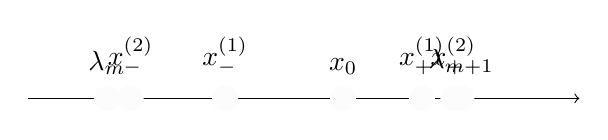
\begin{tikzpicture}
 \draw[->] (-1.5,0) -- (5.5,0); 
 \node[circle, fill=black!1, label=above:$x_{0}$] at (2.5,0) {};
 \uncover<2>{
   \node[circle, fill=black!1, label=above:$x^{(1)}_{-}$] at (1,0) {};
   \node[circle, fill=black!1, label=above:$x^{(1)}_{+}$] at (3.5,0) {};
 }
 \uncover<3>{
   \node[circle, fill=black!1, label=above:$x^{(2)}_{-}$] at (-0.2,0) {};
   \node[circle, fill=black!1, label=above:$x^{(2)}_{+}$] at (3.9,0) {};
   }
 \uncover<4>{
   \node[circle, fill=black!1, label=above:$\lambda_{m}$] at (-.5,0) {};
   \node[circle, fill=black!1, label=above:$\lambda_{m+1}$] at (4,0) {};
 }
\end{tikzpicture}

\end{frame}



\begin{frame}
\frametitle{Fast and secure iterative method}

\begin{de}[Laguerre's iteration]
  If $mlt(\lambda_m)=mlt(\lambda_{m+1})=1$ then
  \begin{align*}
    x_{+}^{(k)} &= L_{+}^k(x)=L_{+}(L_{+}(\dots(x_{0})))\\
    x_{-}^{(k)} &= L_{-}^k(x)=L_{-}(L_{-}(\dots(x_{0})))
  \end{align*}
  else we have a similar expression.
\end{de} 

\pause

We can prove that

\begin{equation*}
  \lambda_m \leftarrow \dots x_{-}^{(2)} < x_{-}^{(1)} < x_{0} < x_{+}^{(1)} < x_{+}^{(2)} \dots \rightarrow \lambda_{m+1}
\end{equation*}
  
\pause

So Laguerre's method is \textcolor{green}{secure}.

\end{frame}

%%%
%DIMOSTRAZIONE
%%%

\begin{frame}
\frametitle{Fast and secure iterative method}

We also have un important property:

\begin{te}
  If we choose\symbolfootnote[1]{ for $x_0 < \lambda_{m+1}$ s.t. 
$sign( \frac{f^{'}(x_0)}{f(x_0)} ) = sign(\lambda_m - x_0)$ we have 
$\{ x_{+}^{(k)} \}_{k=1,\dots}$ conv. mon. cubic to $\lambda_{m+1}$ } $\lambda_m < x_0$ s.t. 
$sign( \frac{f^{'}(x_0)}{f(x_0)} ) = sign(\lambda_m - x_0)$ then 
$\{ x_{-}^{(k)} \}_{k=1,\dots}$ converge monotonically in asymptotically 
cubic rate to $\lambda_m$. 
\end{te}

\pause

So we can exactly define a $\fbox{neighborood ``near'' $\lambda$ }$ and in it we
have cubic rate convergence (much, much faster then \textcolor{red}{bisection}) 

\pause

The Laguerre's method is \textcolor{green}{fast}.

\end{frame}

\begin{frame}
\frametitle{Fast and secure iterative method}

It's clear that we need a powerfull method to obtain $x_{0}$ and an algorithm to 
estimate $mlt(\lambda_m)$. \\
\emph{Overstimate} $mlt(\lambda_m)$ (as we can read in \cite{MR1289159}) causes no trouble, so the most importan aspects of our calculation are: 

\fbox{\setlength{\itemsep}{0pt}
\begin{Bitemize}[t]
\item Good $x_{0}$.
\item Good evaluation of $L_{\pm}(x)$.
\end{Bitemize}}

\end{frame}


\section{Good evaluation of $L_{\pm}(x)$}

\begin{frame}
  \frametitle{Three term recurrence}
  For a generic $x\in\R$ we call $\rho_n(x) = \deter{T_n-x S_n}$,
  and $\rho_{n-1}(x) = \deter{T_{n-1}-x S_{n-1}}$, with $T_{n-1}$ leading principal submatrix. 

  We have

  \begin{align*}
    \rho_0 &:= 1\, \text{, } \rho_1:=t_{1,1}- x s_{1,1} \\
    \rho_i &:= (t_{i,i}- x s_{i,i})\textcolor{blue}{\rho_{i-1}} - (t_{i-1,i}-x s_{i-1,i})^2 \textcolor{cyan}{\rho_{i-2}}\, \text{, } i=2,3,\dots,n
  \end{align*}

\end{frame}

\begin{frame}
  \frametitle{Three term recurrence}

  We can proove it with the \emph{Laplace expansion} (e.g. $n=4$)

  \begin{align*}
    T_4 - x S_4  &= \begin{pmatrix} 
      a & b & 0 & \textcolor{green}{0}\\
      b & c & d & \textcolor{green}{0}\\
      0 & d & e & \textcolor{green}{f}\\
      0 & 0 & f & \textcolor{green}{g}
    \end{pmatrix} \\
    det \Big( T_4 - \lambda S_4 \Big) &= g \begin{bmatrix}
      a & b & 0\\
      b & c & d\\
      0 & d & e
    \end{bmatrix} -f \begin{bmatrix}
      a & b & 0\\
      b & c & d\\
      \textcolor{green}{0} & \textcolor{green}{0} & \textcolor{green}{f}
    \end{bmatrix}\\
    &= g \begin{bmatrix} 
      a & b & 0\\
      b & c & d\\
      0 & d & e
    \end{bmatrix} - f^2 \begin{bmatrix} a & b \\ b & c \end{bmatrix}
  \end{align*}

\end{frame}

\begin{frame}
  \frametitle{Three term recurrence}

  We can proove it with the \emph{Laplace expansion} (e.g. $n=4$)

  \begin{align*}
    T_4 - x S_4  &= \begin{pmatrix} 
      \textcolor{cyan}{a} & \textcolor{cyan}{b} & \textcolor{blue}{0} & 0\\
      \textcolor{cyan}{b} & \textcolor{cyan}{c} & \textcolor{blue}{d} & 0\\
      \textcolor{blue}{0} & \textcolor{blue}{d} & \textcolor{blue}{e} & f\\
      0 & 0 & f & g
    \end{pmatrix} \\
    det \Big( T_4 - \lambda S_4 \Big) &= g \begin{bmatrix}
      \textcolor{cyan}{a} & \textcolor{cyan}{b} & \textcolor{blue}{0}\\
      \textcolor{cyan}{b} & \textcolor{cyan}{c} & \textcolor{blue}{d}\\
      \textcolor{blue}{0} & \textcolor{blue}{d} & \textcolor{blue}{e}
    \end{bmatrix} -f \begin{bmatrix}
      \textcolor{cyan}{a} & \textcolor{cyan}{b} & 0\\
      \textcolor{cyan}{b} & \textcolor{cyan}{c} & d\\
      0 & 0 & f
    \end{bmatrix}\\
    &= g \begin{bmatrix} 
      \textcolor{cyan}{a} & \textcolor{cyan}{b} & \textcolor{blue}{0}\\
      \textcolor{cyan}{b} & \textcolor{cyan}{c} & \textcolor{blue}{d}\\
      \textcolor{blue}{0} & \textcolor{blue}{d} & \textcolor{blue}{e}
    \end{bmatrix} - f^2 \begin{bmatrix} 
      \textcolor{cyan}{a} & \textcolor{cyan}{b} \\ 
      \textcolor{cyan}{b} & \textcolor{cyan}{c} 
    \end{bmatrix}
  \end{align*}

\end{frame}


\begin{frame}
  \frametitle{Three term recurrence}

  \begin{os}
    If $x = \lambda$ then $\rho_n(\lambda)=\effe{(T_n,S_n)}{\lambda}=f$
  \end{os}

  \begin{os}
    $\rho_0,\rho_1,\dots,\rho_n$ i a \textcolor{blue}{\emph{Sturm sequence}} of polynomials so, $\forall x\in\R$, we have

    \begin{align*}
      \kappa(x) &:= \text{\# eigenvalues less then } x \\
      \kappa(x) &= \textcolor{blue}{\text{\# consecutive sign changes in }} \{ \rho_i \}_{i=0,\dots,n}
    \end{align*}
  \end{os}

  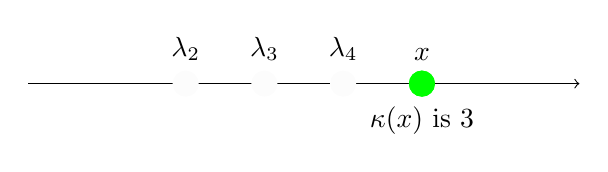
\begin{tikzpicture}
    \draw[->] (-5,0) -- (2,0);
    \node[circle, fill=black!1, label=above:$\lambda_2$] at (-3,0) {};
    \node[circle, fill=black!1, label=above:$\lambda_3$] at (-2,0) {};
    \node[circle, fill=black!1, label=above:$\lambda_4$] at (-1,0) {};
    \node[circle, fill=green, label=above:$x$] at (0,0) {};
    \node[circle, fill=green, label=below:$\kappa(x)\text{ is } 3$] at (0,0) {};
  \end{tikzpicture}

  %We will see that $\kappa(x)$ is a fondamental
  

\end{frame}

%%%
%%%
%%%

\section{Good initial point}

\begin{frame}
\frametitle{Searching $x_0$}

\begin{Bdescription}
  \item [We want:]
  \fbox{\setlength{\itemsep}{0pt}%
  \begin{Bitemize}[t]
  \item Fast and secure iterative method.
  \item \textcolor{blue}{Starting points for our method}.
  \item Scalability.
  \end{Bitemize}}
  
  \item [We have:]
  \fbox{\setlength{\itemsep}{0pt}%
  \begin{Bitemize}[t]
  \item Laguerre's method.
  \item Cuppen's divide and conquer method.
  \item Symmetric tridiagonal matrices.
  \end{Bitemize}}

  \item [We add:]
  \fbox{\setlength{\itemsep}{0pt}%
  \begin{Bitemize}[t]
  \item Unreducible condition.
  \item Dynamic programming (Bottom-up).
  \item Efficient matrix storing.
  \end{Bitemize}}
\end{Bdescription}
\end{frame}

\begin{frame}
  \frametitle{Ideas:}
  If $n=1$ we have $t\cdot v=\lambda\cdot s\cdot v$. $s\ne 0$, so 
  $\lambda= \frac{t}{s}$.\\
  
  \pause
  
  If $n=2$ we have $\begin{bmatrix}t_{1,1}&t_{1,2}\\ t_{2,1} & t_{2,2}\end{bmatrix} \begin{bmatrix}v_{1} \\ v_{2}\end{bmatrix} = \lambda \begin{bmatrix}s_{1,1} & s_{1,2}\\ s_{2,1} & s_{2,2}\end{bmatrix} \begin{bmatrix}v_{1} \\ v_{2}\end{bmatrix}$


\end{frame}


\begin{frame}
  \frametitle{Ideas:}
  If $n=1$ we have $t\cdot v=\lambda\cdot s\cdot v$. $s\ne 0$, so 
  $\lambda= \frac{t}{s}$.\\
  
  If $n=2$ we have $\begin{bmatrix}t_{1,1}&t_{1,2}\\ t_{2,1} & t_{2,2}\end{bmatrix} \begin{bmatrix}v_{1} \\ v_{2}\end{bmatrix} = \lambda \begin{bmatrix}s_{1,1} & s_{1,2}\\ s_{2,1} & s_{2,2}\end{bmatrix} \begin{bmatrix}v_{1} \\ v_{2}\end{bmatrix}$
  
  
  calling\symbolfootnote[1]{$\alpha=,\beta=,\gamma=$.} 

  \begin{equation*}
    S^{-1}T = \delta^{-1} \cdot \Big( \begin{matrix} \alpha & \gamma \\ \gamma & \beta \end{matrix}\Big)
  \end{equation*}

  we resolve $det[ S^{-1}T - \lambda I ]=0$ with

  \begin{equation*}
    \lambda_{1,2} = \frac{1}{2\delta}  
  \big( \alpha+\beta \pm \sqrt{ \alpha^2 + \beta^2 + 
  \gamma^2 - \alpha\beta } \big)
  \end{equation*}

\end{frame}

\begin{frame}
  \frametitle{Ideas:}

  And if $n=4$?
  
  \begin{equation*}
    \begin{bmatrix}
      a & b\\
      c & d
    \end{bmatrix}
  \end{equation*}


\end{frame}

\begin{frame}
\frametitle{Split}

Consider $(\hat T, \hat S)$ with

\begin{align*}
 \hat T &= \begin{bmatrix} T_{0} & 0\\ 0 & T_{1} \end{bmatrix}\\
 \hat S &= \begin{bmatrix} S_{0} & 0\\ 0 & S_{1} \end{bmatrix}\\
\end{align*}

and let be

\begin{equation*}
  \hat\lambda_1 \le \hat\lambda_2 \le \dots \le \hat\lambda_n
\end{equation*}

eigenvalues of $(\hat T, \hat S)$, then

\end{frame}

\begin{frame}
\frametitle{Split}

\begin{te}[A sort of ``interlacing'']

\begin{align*}
  -\infty < &\lambda_1 \le \hat\lambda_1 \\
  \hat\lambda_{i-1} \le &\lambda_i \le \hat\lambda_{i+1} \\
  \hat\lambda_n \le &\lambda_n < \infty
\end{align*}

with $i=2,3,\dots,n-1$.

\end{te}

\begin{os}
It's possible that

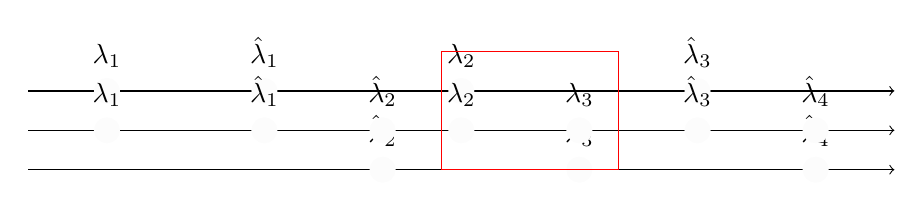
\begin{tikzpicture}
  \uncover<1>{
    \draw[->] (-2,0) -- (9,0); 
    \node[circle, fill=black!1, label=above:$\lambda_{1}$] at (-1,0) {};
    \node[circle, fill=black!1, label=above:$\hat\lambda_{1}$] at (1,0) {};
    \node[circle, fill=black!1, label=above:$\lambda_{2}$] at (3.5,0) {};
    \node[circle, fill=black!1, label=above:$\hat\lambda_{3}$] at (6.5,0) {};
    %%%
    \draw[->] (-2,-1) -- (9,-1); 
    \node[circle, fill=black!1, label=above:$\hat\lambda_{2}$] at (2.5,-1) {};
    \node[circle, fill=black!1, label=above:$\lambda_{3}$] at (5,-1) {};
    \node[circle, fill=black!1, label=above:$\hat\lambda_{4}$] at (8,-1) {};
  }
  \uncover<2,3>{
    \draw[->] (-2,-.5) -- (9,-.5); 
    \node[circle, fill=black!1, label=above:$\lambda_{1}$] at (-1,-.5) {};
    \node[circle, fill=black!1, label=above:$\hat\lambda_{1}$] at (1,-.5) {};
    \node[circle, fill=black!1, label=above:$\lambda_{2}$] at (3.5,-.5) {};
    \node[circle, fill=black!1, label=above:$\hat\lambda_{3}$] at (6.5,-.5) {};
    \node[circle, fill=black!1, label=above:$\hat\lambda_{2}$] at (2.5,-.5) {};
    \node[circle, fill=black!1, label=above:$\lambda_{3}$] at (5,-.5) {};
    \node[circle, fill=black!1, label=above:$\hat\lambda_{4}$] at (8,-.5) {};
  }
  \uncover<3>{
    \draw[red] (3.25,.5) rectangle (5.5,-1);
    }
\end{tikzpicture}


\end{os}

\end{frame}

\begin{frame}
\frametitle{Split}

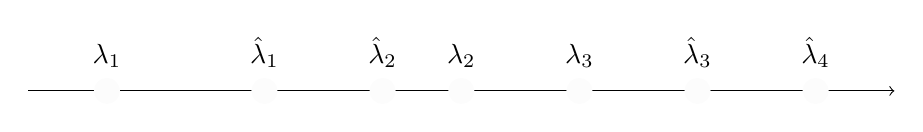
\begin{tikzpicture}
\draw[->] (-2,-.5) -- (9,-.5); 
\node[circle, fill=black!1, label=above:$\lambda_{1}$] at (-1,-.5) {};
\node[circle, fill=black!1, label=above:$\hat\lambda_{1}$] at (1,-.5) {};
\node[circle, fill=black!1, label=above:$\lambda_{2}$] at (3.5,-.5) {};
\node[circle, fill=black!1, label=above:$\hat\lambda_{3}$] at (6.5,-.5) {};
\node[circle, fill=black!1, label=above:$\hat\lambda_{2}$] at (2.5,-.5) {};
\node[circle, fill=black!1, label=above:$\lambda_{3}$] at (5,-.5) {};
\node[circle, fill=black!1, label=above:$\hat\lambda_{4}$] at (8,-.5) {};
\end{tikzpicture}

So we can't 

\end{frame}

\frame{
\begin{center}
Grazie per l'attenzione.
\end{center}
}



%%%
%%%
%%%
\end{document}
